\begin{figure}[tbp]
\centering
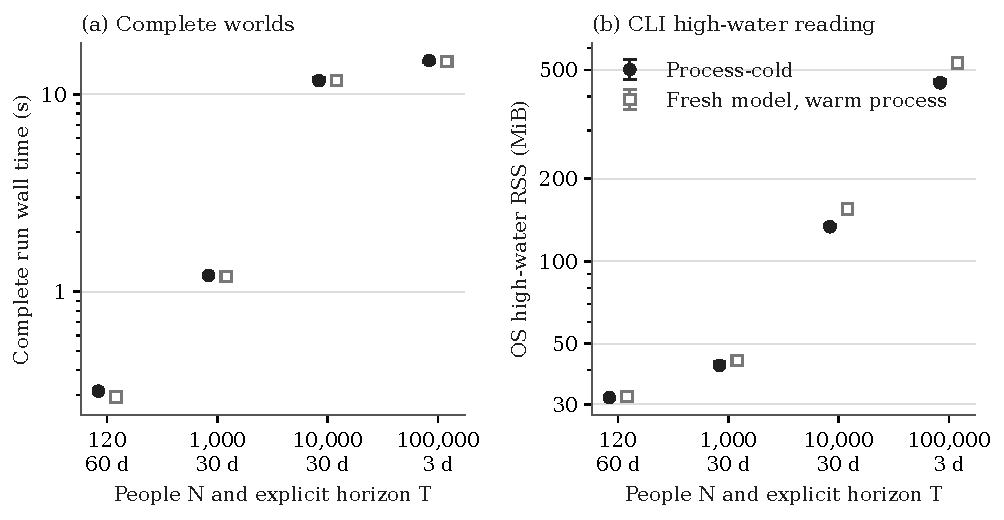
\includegraphics[width=\linewidth]{figures/results/benchmark_workloads.pdf}
\caption{Complete runs including output hashes, final manifests and measurement readback, excluding process launch, on Apple M2 Pro/macOS 26.6/Python 3.14.6, benchmark source 3d67a62e6eb2. Points are medians and bars min--max of three child-process repeats; every warm repeat initializes a fresh full model. Horizons differ explicitly, so the populations are not a common-horizon scaling series. CLI RSS is OS high-water read before final output hashes; warm points inherit prior high-water and allocator state. The whole-child guardian peak is separately retained and used for conservative memory planning. All normal daily modules and full-state output are retained. This is software resource evidence, not organizational efficiency.}
\label{fig:benchmark-workloads}
\end{figure}
\begin{figure}[tbp]
\centering
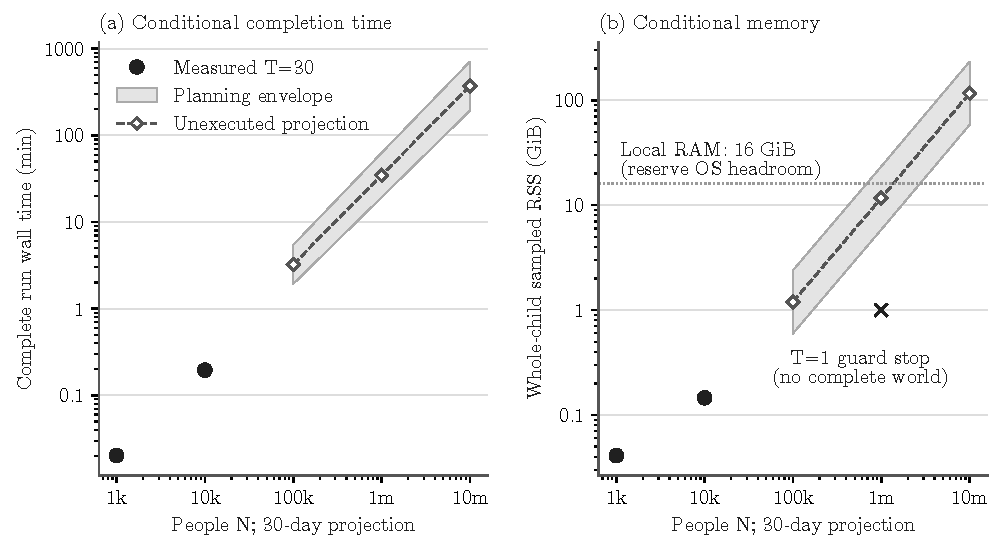
\includegraphics[width=\linewidth]{figures/results/benchmark_projection.pdf}
\caption{Source 3d67a62e6eb2; black circles are complete measured 30-day workloads, hollow diamonds/dashes are unexecuted 30-day projections. Hatched bands are deliberately broad structural planning envelopes, not confidence intervals or guaranteed limits. A fitted N plus NT memory/output model and observed phase rates with logarithmic heap/sort growth give these scenarios. Memory fits the median whole-child guardian peaks sampled every 50 ms, including both fresh models and final hashing, rather than a reset per-world high-water. Four measured cells (including 100,000 people for three days) fit local coefficients; they do not independently validate large-scale prediction. The cross marks the actual million-person one-day RSS stop, not a completed world's peak. All projected thirty-day requests exceed the default event limit; no completed results or cloud performance are implied.}
\label{fig:benchmark-projection}
\end{figure}
\begin{figure}[tbp]
\centering
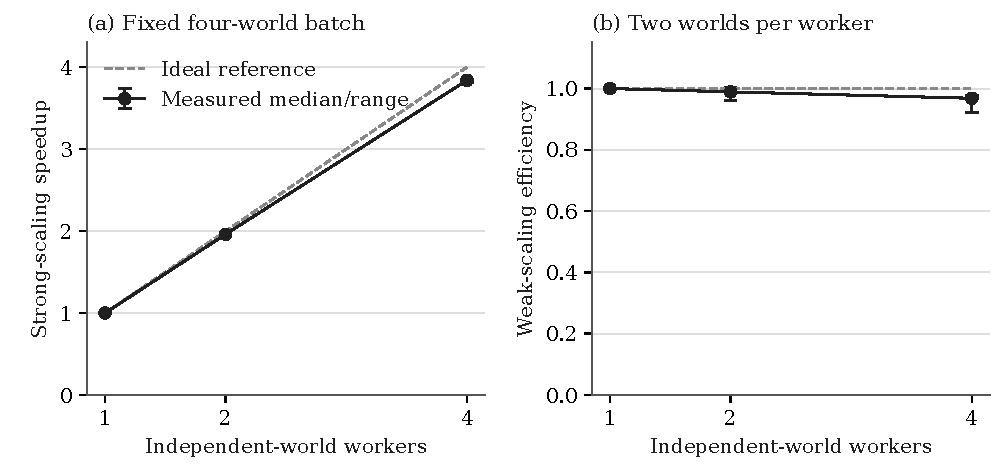
\includegraphics[width=\linewidth]{figures/results/benchmark_parallel.pdf}
\caption{Benchmark source 3d67a62e6eb2; N=1,000, T=30, full modules and outputs. Strong scaling holds four matched worlds fixed; weak scaling holds two worlds per worker. Points are medians and bars min--max across three batches; dashed lines show ideal references. Launch, execution and monitoring enter batch wall time. Each of eight world IDs has exactly one final-state SHA-256 across worker counts and repeats. These are same-platform deterministic checks, not external validation, single-world MPI scaling or a GPU benchmark.}
\label{fig:benchmark-parallel}
\end{figure}
